\documentclass{report}
% Include all project wide packages here.
\usepackage{fullpage}
\usepackage[style=ieee]{biblatex}
\usepackage[dutch]{babel}

\renewcommand{\familydefault}{\sfdefault}

\setmainfont[Ligatures=TeX]{Myriad Pro}
\setmathfont{Asana Math}
\setmonofont{Lucida Console}

\usepackage{titlesec, blindtext, color}
\definecolor{gray75}{gray}{0.75}
\newcommand{\hsp}{\hspace{20pt}}
\titleformat{\chapter}[hang]{\Huge\bfseries}{\thechapter\hsp\textcolor{gray75}{|}\hsp}{0pt}{\Huge\bfseries}
\renewcommand{\familydefault}{\sfdefault}
\renewcommand{\arraystretch}{1.2}
\setlength\parindent{0pt}

%For code listings
\definecolor{black}{rgb}{0,0,0}
\definecolor{browntags}{rgb}{0.65,0.1,0.1}
\definecolor{bluestrings}{rgb}{0,0,1}
\definecolor{graycomments}{rgb}{0.4,0.4,0.4}
\definecolor{redkeywords}{rgb}{1,0,0}
\definecolor{bluekeywords}{rgb}{0.13,0.13,0.8}
\definecolor{greencomments}{rgb}{0,0.5,0}
\definecolor{redstrings}{rgb}{0.9,0,0}
\definecolor{purpleidentifiers}{rgb}{0.01,0,0.01}


\lstdefinestyle{csharp}{
language=[Sharp]C,
showspaces=false,
showtabs=false,
breaklines=true,
showstringspaces=false,
breakatwhitespace=true,
escapeinside={(*@}{@*)},
columns=fullflexible,
commentstyle=\color{greencomments},
keywordstyle=\color{bluekeywords}\bfseries,
stringstyle=\color{redstrings},
identifierstyle=\color{purpleidentifiers},
basicstyle=\ttfamily\small}

\lstdefinestyle{c}{
language=C,
showspaces=false,
showtabs=false,
breaklines=true,
showstringspaces=false,
breakatwhitespace=true,
escapeinside={(*@}{@*)},
columns=fullflexible,
commentstyle=\color{greencomments},
keywordstyle=\color{bluekeywords}\bfseries,
stringstyle=\color{bluestrings},
identifierstyle=\color{purpleidentifiers}
}

\lstdefinestyle{vhdl}{
language=VHDL,
showspaces=false,
showtabs=false,
breaklines=true,
showstringspaces=false,
breakatwhitespace=true,
escapeinside={(*@}{@*)},
columns=fullflexible,
commentstyle=\color{greencomments},
keywordstyle=\color{bluekeywords}\bfseries,
stringstyle=\color{redstrings},
identifierstyle=\color{purpleidentifiers}
}

\lstdefinestyle{xaml}{
language=XML,
showspaces=false,
showtabs=false,
breaklines=true,
showstringspaces=false,
breakatwhitespace=true,
escapeinside={(*@}{@*)},
columns=fullflexible,
commentstyle=\color{greencomments},
keywordstyle=\color{redkeywords},
stringstyle=\color{bluestrings},
tagstyle=\color{browntags},
morestring=[b]",
  morecomment=[s]{<?}{?>},
  morekeywords={xmlns,version,typex:AsyncRecords,x:Arguments,x:Boolean,x:Byte,x:Char,x:Class,x:ClassAttributes,x:ClassModifier,x:Code,x:ConnectionId,x:Decimal,x:Double,x:FactoryMethod,x:FieldModifier,x:Int16,x:Int32,x:Int64,x:Key,x:Members,x:Name,x:Object,x:Property,x:Shared,x:Single,x:String,x:Subclass,x:SynchronousMode,x:TimeSpan,x:TypeArguments,x:Uid,x:Uri,x:XData,Grid.Column,Grid.ColumnSpan,Click,ClipToBounds,Content,DropDownOpened,FontSize,Foreground,Header,Height,HorizontalAlignment,HorizontalContentAlignment,IsCancel,IsDefault,IsEnabled,IsSelected,Margin,MinHeight,MinWidth,Padding,SnapsToDevicePixels,Target,TextWrapping,Title,VerticalAlignment,VerticalContentAlignment,Width,WindowStartupLocation,Binding,Mode,OneWay,xmlns:x}
}

%defaults
\lstset{
basicstyle=\ttfamily\small,
extendedchars=false,
numbers=left,
numberstyle=\ttfamily\tiny,
stepnumber=1,
tabsize=4,
numbersep=5pt
}

\title{Resultaten}
\author{J.F.J. Blom}
\date{\today}
\begin{document}
\section*{Resultaten en Discussie}
Er zijn drie verschillende metingen verricht, kalibratiemeting, onbekende afstandsmeting en de lineariteitsmeting. Deze metingen zijn drie keer gedaan en dus zijn de meetresultaten ook drie keer weergeven en geanalyseerd.
\subsection*{Kalibratie}
\subsubsection*{Meting 1}
Hieronder zijn de meetresultaten van de eerste kalibratiemeting te zien. Deze meting is maar vijf keer uitgevoerd terwijl het de bedoeling was dat deze tien keer werd uitgevoerd, maar bij een enkel groepje is de opdracht verkeerd geïnterpreteerd.

\begin{table}
\begin{center}
\begin{tabular}{| l| c|}
\hline
    & Kalibratie 10 cm \\
\hline
   Meting 1 (s) & 1.031 \\
\hline
   Meting 2 (s) & 1.042 \\
\hline
   Meting 3 (s) & 1.042 \\
\hline
   Meting 4 (s) & 1.046 \\
\hline
   Meting 5 (s) & 1.045 \\
\hline
\end{tabular}
\caption{TODO caption}
\end{center}
\end{table}

\begin{center}
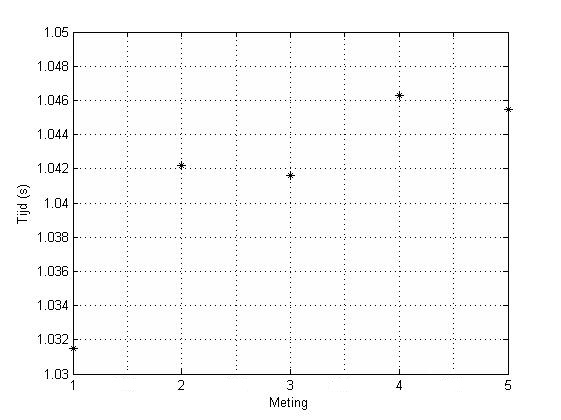
\includegraphics[width=150mm] {grafiekmeetresultaten1.jpg}
\end{center}

$$ t_{gem}=\frac{\sum_{i=1}^{n}t_i}{n} = 1.041 s$$

$$ v_{gem} = \frac{s}{t_{gem}} = 9.602 cm/s$$

$$ s(t) = \sqrt{\frac{\sum_{i=1}^{n}( t_i-t_{gem})^2}{n-1}} = 0.582 s$$

$$ u(t) = \frac{s}{\sqrt{n}} = \sqrt{\frac{\sum_{i=1}^{n}( t_i-t_{gem})^2}{n(n-1)}} = 0.003 s$$ 

$$ u(v) = \sqrt{\left (\frac{\partial v }{\partial t }\right)^2 u(t)^2 + \left (\frac{\partial v }{\partial s }\right)^2 u(s)^2} = \sqrt{\left (\frac{s }{{t_{gem}}^2 }\right)^2 u(t)^2 + \left (\frac{1}{t_{gem} }\right)^2 u(s)^2} = 0.054 cm/s$$


\subsubsection*{Meting 2}
\begin{table}
\begin{center}
\begin{tabular}{| l| c|}
\hline
    & Kalibratie 10 cm \\
\hline
   Meting 1 (s) & 1.128\\
\hline
   Meting 2 (s) & 1.127\\
\hline
   Meting 3 (s) & 1.137\\
\hline
   Meting 4 (s) & 1.142\\
\hline
   Meting 5 (s) & 1.130 \\
\hline
   Meting 6 (s) & 1.136\\
\hline
   Meting 7 (s) & 1.140\\
\hline
   Meting 8 (s) & 1.130\\
\hline
   Meting 9 (s) & 1.131\\
\hline
   Meting 10 (s) & 1.145 \\
\hline
\end{tabular}
\caption{TODO caption}
\end{center}
\end{table}

\begin{figure}[H]
\begin{center}
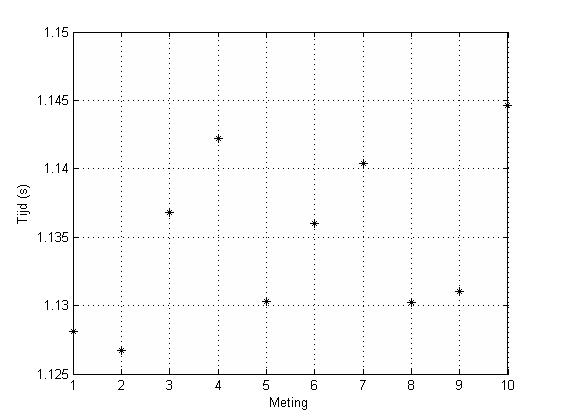
\includegraphics[width=150mm] {grafiekmeetresultaten2.jpg}
\caption{TODO caption}
\end{center}
\end{figure}

$$ t_{gem}=\frac{\sum_{i=1}^{n}t_i}{n} = 1.135 s$$

$$ v_{gem} = \frac{s}{t_{gem}} = 8.813 cm/s$$

$$ s = \sqrt{\frac{\sum_{i=1}^{n}( t_i-t_{gem})^2}{n-1}} = 0.006 s$$

$$ u = \frac{s}{\sqrt{n}} = \sqrt{\frac{\sum_{i=1}^{n}( t_i-t_{gem})^2}{n(n-1)}} = 0.002 s$$

$$ u(v) = \sqrt{\left (\frac{\partial v }{\partial t }\right)^2 u(t)^2 + \left (\frac{\partial v }{\partial s }\right)^2 u(s)^2} = \sqrt{\left (\frac{s }{{t_{gem}}^2 }\right)^2 u(t)^2 + \left (\frac{1}{t_{gem} }\right)^2 u(s)^2} = 0.047 cm/s$$

\subsubsection*{Meting 3}
\begin{table}
\begin{center}
\begin{tabular}{| l| c|}
\hline
    & Kalibratie 10 cm \\
\hline
   Meting 1 (s) & 1.170 \\
\hline
   Meting 2 (s) & 1.173 \\
\hline
   Meting 3 (s) & 1.142 \\
\hline
   Meting 4 (s) & 1.146 \\
\hline
   Meting 5 (s) & 1.164 \\
\hline
   Meting 6 (s) & 1.167 \\
\hline
   Meting 7 (s) & 1.171 \\
\hline
   Meting 8 (s) & 1.167\\
\hline
   Meting 9 (s) & 1.156\\
\hline
   Meting 10 (s) & 1.152\\
\hline
\end{tabular}
\caption{TODO caption}
\end{center}
\end{table}

\begin{figure}
\begin{center}
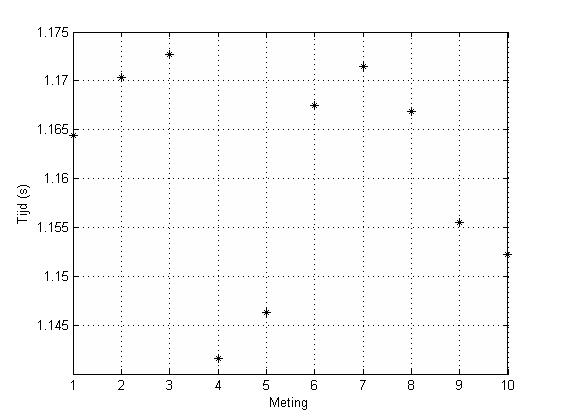
\includegraphics[width=150mm] {grafiekmeetresultaten3.jpg}
\caption{TODO caption}
\end{center}
\end{figure}
Hierboven zijn de meetresultaten van de kalibratiemeting in een diagram gezet. Hier zijn goed de verschillen tussen de metingen te zien.

$$ t_{gem}=\frac{\sum_{i=1}^{n}t_i}{n} = 1.161 s$$

$$ v_{gem} = \frac{s}{t_{gem}} = 8.614 cm/s$$

$$ s = \sqrt{\frac{\sum_{i=1}^{n}( t_i-t_{gem})^2}{n-1}} = 0.011 s$$

$$ u = \frac{s}{\sqrt{n}} = \sqrt{\frac{\sum_{i=1}^{n}( t_i-t_{gem})^2}{n(n-1)}} = 0.004 s$$

$$ u(v) = \sqrt{\left (\frac{\partial v }{\partial t }\right)^2 u(t)^2 + \left (\frac{\partial v }{\partial s }\right)^2 u(s)^2} = \sqrt{\left (\frac{s}{{t_{gem}}^2 }\right)^2 u(t)^2 + \left (\frac{1}{t_{gem} }\right)^2 u(s)^2} =0.050 cm/s$$

\subsection*{Onbekende afstand}
\subsubsection*{Meting 1}
Hieronder zijn de meetresultaten te zien van de onbekende afstandsmeting. Om de snelheid te kunnen bepalen moet er een afstand bekend zijn. Deze afstand is gemeten en deze is 23.4 cm.
\begin{table}
\begin{center}
\begin{tabular}{| l| c|}
\hline
    & Onbekende afstand 23.4 cm\\
\hline
   Meting 1 (s) & 2.526 \\
\hline
   Meting 2 (s) & 2.531 \\
\hline
   Meting 3 (s) & 2.518 \\
\hline
   Meting 4 (s) & 2.515 \\
\hline
   Meting 5 (s) & 2.522 \\
\hline
 \end{tabular}
\caption{TODO caption}
\end{center}
\end{table}

De gemiddelde tijd die het kost om de onbekende afstand af te leggen is

$$ t_{gem}=\frac{\sum_{i=1}^{n}t_i}{n} = 2.523 s$$ 

Deze tijd kunnen we gebruiken in combinatie met de gemiddelde snelheid die we eerder hebben vastgesteld om de onbekende afstand te berekenen

$$ s = v_{gem} \cdot t_{gem}$$
$$ = 9.602 cm/s \cdot 2.523 s = 24.23 cm$$

\subsubsection*{Meting 2}

\subsubsection*{Meting 3}

\subsection*{Lineariteit}
\subsubsection*{Meting 1}
Hieronder zijn de meetresultaten te zien van de lineariteitsmeting. Doormiddel van de meetresultaten en de afstand is de gemiddelde snelheid uitgerekend. Onder de tabel en op de volgende pagina zijn deze gegevens in diagrammen gezet, waardoor de afwijkingen in lineariteit beter te zien zijn. 
\begin{table}
\begin{center}
\begin{tabular}{| l| c| c| c| c| c|}
\hline
   & 5 cm & 10 cm & 15 cm & 20 cm & 25 cm\\
\hline
   Meting 1 (s) & 0.542 & 1.092 & 1.638 & 2.218 & 2.728 \\
\hline
 \end{tabular}
\caption{TODO caption}
\end{center}
\end{table}

\begin{figure}
\begin{center}
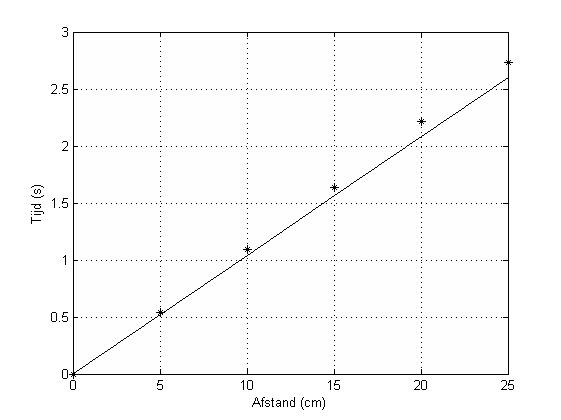
\includegraphics[width=150mm] {Lineariteitsmeting1.jpg}
\caption{TODO caption}
\end{center}
\end{figure}

\subsubsection*{Meting 2}
\begin{figure}
\begin{center}
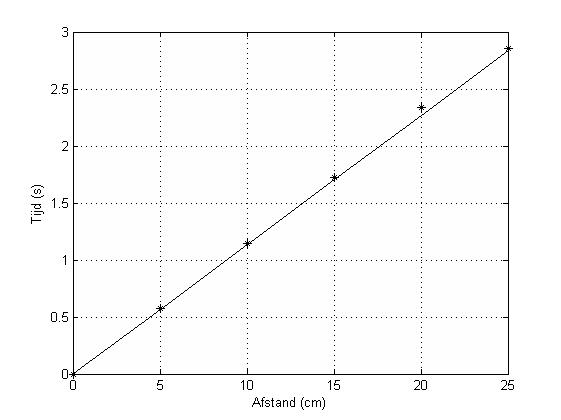
\includegraphics[width=150mm] {Lineariteitsmeting2.jpg}
\caption{TODO caption}
\end{center}
\end{figure}

\subsubsection*{Meting 3}
\begin{figure}
\begin{center}
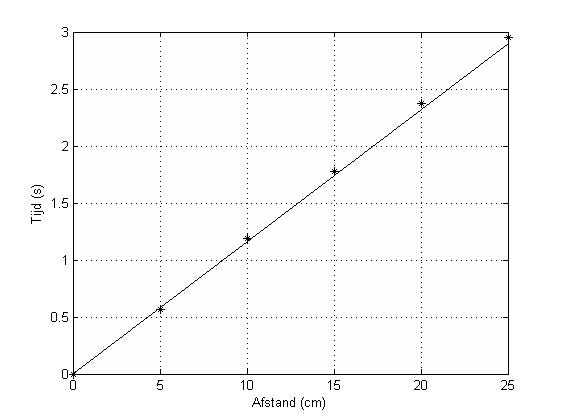
\includegraphics[width=150mm] {Lineariteitsmeting3.jpg}
\caption{TODO caption}
\end{center}
\end{figure}
\newpage
\section*{Conclusie}

\end{document}